\documentclass[USenglish,oneside,twocolumn]{article}
\usepackage{color}
\usepackage[hyphens]{url}
\usepackage{longtable}
\usepackage{graphicx}
\usepackage{enumitem}
\usepackage{pdfpages}
\usepackage{adjustbox}
%\usepackage{hyperref}

\usepackage[utf8]{inputenc}%(only for the pdftex engine)
%\RequirePackage[no-math]{fontspec}%(only for the luatex or the xetex engine)
\usepackage[big]{dgruyter_NEW}
 
\hyphenation{Isa-bela}

\DOI{foobar}

\cclogo{
\includegraphics{by-nc-nd.pdf}}

% Format a participant quotation.
\newcommand{\pquote}[2]{
\begin{quotation}
\noindent #1:~\textit{``#2''}
\end{quotation}
}
  
\begin{document}
   \author*[1]{Author 1}

  \author[2]{Author 2}

  \author[3]{Author 3}

  \author[4]{Author 4}

  \author[5]{Author 5}
  
  \author[6]{Author 6}

  \affil[1]{Affiliation of Author 1, E-mail: \mbox{author1@affiliation.edu}}
  \affil[2]{Affiliation of Author 2, E-mail: \mbox{author2@affiliation.edu}}
  \affil[3]{Affiliation of Author 3, E-mail: \mbox{author3@affiliation.edu}}
  \affil[4]{Affiliation of Author 4, E-mail: \mbox{author4@affiliation.edu}}
  \affil[5]{Affiliation of Author 5, E-mail: \mbox{author5@affiliation.edu}}
  \affil[6]{Affiliation of Author 6, E-mail: \mbox{author6@affiliation.edu}}
%  \author*[1]{Linda Lee}
%
%  \author[2]{David Fifield}
%
%  \author[3]{Nathan Malkin}
%
%  \author[4]{Ganesh Iyer}
%
%  \author[5]{Serge Egelman}
%  
%  \author[6]{David Wagner}
%
%  \affil[1]{University of California Berkeley, E-mail: \mbox{lnl@cs.berkeley.edu}}
%
%  \affil[2]{University of California Berkeley, E-mail: \mbox{fifield@cs.berkeley.edu}}
%
%  \affil[3]{University of California Berkeley, E-mail: \mbox{nmalkin@cs.berkeley.edu}}
%
%  \affil[4]{University of California Berkeley, E-mail: \mbox{ganesh.v@berkeley.edu}}
%  
%  \affil[5]{University of California Berkeley and International Computer Science Institute, E-mail: \mbox{egelman@cs.berkeley.edu}}
%   
%  \affil[6]{University of California Berkeley, E-mail: \mbox{daw@cs.berkeley.edu}}

  \title{\huge A Better (One-Line!) Title Here}

  \runningtitle{Ugh!}

  %\subtitle{...}

  \begin{abstract}
{
We evaluate, design, and test the Tor Launcher interface by
placing users in simulated censorship environments, instructing them to use Tor
to circumvent censorship, and measuring their interface interactions.
A 16-participant qualitative study examines user assumptions and common mistakes.
We use the results as feedback to redesign the configuration interface.
A 114-participant quantitative study shows that our design changes result in
a significant reduction in time. We conclude with recommendations for changes 
to the current interface as well as alternative solutions.}
\end{abstract}
  \keywords{Usable Security, User Studies, Tor, Security, Censorship, Anonymity}
%  \classification[PACS]{}
 % \communicated{...}
 % \dedication{...}

  \journalname{Proceedings on Privacy Enhancing Technologies}
\DOI{Editor to enter DOI}
  \startpage{1}
  \received{..}
  \revised{..}
  \accepted{..}

  \journalyear{2015}
  \journalvolume{2015}
  \journalissue{2}

\maketitle

\section{Introduction}

Tor~\cite{dingledine2004tor} is an anonymity network that routes Internet traffic through a series of relays 
that make it difficult to observe the source and destination. 
Tor Browser~\cite{torbrowser}, a modified Firefox browser with a built-in Tor client, 
is the recommended way to use Tor. Tor Launcher is a Tor Browser component that
starts, stops, and otherwise controls the underlying Tor processes.
Tor Launcher's graphical user interface asks the user to configure
bridges, pluggable transports, and proxies to make a connection to Tor (we refer to as the ``configuration interface'' throughout this paper). This is the object of our study. 

We start by introducing terms (section~\ref{sec:background}) and, 
describing the experimental setup (section~\ref{sec:environments}). 
Then we report of user observations and interviews (section~\ref{sec:qualitative}),
list design principles and interface changes (section~\ref{redesign}),
state evaluation criteria for gauging the succcessfulness of an interface (section~\ref{sec:eval}), 
measure the impact of changes in the quantitative experiment in section~\ref{sec:quantitative}, 
testing measured the impact of the design changes (Section~\ref{sec:quantitative}, and
discuss user behaviors (section~\ref{sec:discussion}).
We end with limitations (section~\ref{sec:limitations}), 
related work (section~\ref{sec:related}), 
future work (section~\ref{sec:future}), and
a conclusion (section~\ref{sec:conclusion}). 

This paper contributes:
\smallskip
\begin{itemize}
\item an evaluation of the current configuration interface
\item a redesigned configuration interface
\item logs of 114 users' connection attempts
\item failure modes seen during connection attempts
\item recommended interface changes
\item alternative bootstrapping approaches
\end{itemize}
We hope that our work helps users circumvent censorship and connect to Tor. 

%%%%%% LINDA'S PASS UP TO HERE %%%%%%%%%

\section{Background}
\label{sec:background}
This section provides the necessary background the configuration interface relates to Tor, the network components that are involved in censorship circumvention, and the configuration settings are required to bypass levels of Tor-adverse censorship environments. 

\subsection{Bridges, Pluggable Transports, and Proxies} 
Internet censors seek to block network resources through 
a variety of means, such as falsifying DNS responses, blocking IP addresses, 
filtering keywords, and detecting protocols by deep packet inspection.
Censors can block the Tor network by blocking the list of Tor relays, which 
are public. Blocking Tor becomes challenging when
the Tor network is augmented with \emph{bridges} and \emph{pluggable transports}.
Fig.~\ref{fig:topology} illustrates the interacting components.

\begin{figure}
\centering

\includegraphics{topology.pdf}
\caption{
The chain of components involved in connecting to a website over Tor.
Most users do not need a proxy;
similarly only those users who face a censor need a bridge.
In the diagram, ``Tor'' represents all three anonymizing hops through the Tor network.
We have shown the bridge as a separate component
because of the special role it plays.
When a bridge is used, it takes the place of the first Tor hop.
}
\label{fig:topology}
\end{figure}

Bridges are unlisted Tor relays that make it possible for a user to connect
to the Tor network even if a censor blocks all publicly listed Tor relays.
Pluggable transports are special protocols that run on bridges and obfuscate
Tor's network protocol to make it difficult to detect. 
Configuring a bridge requires providing one or more
``bridge lines,'' a specification of a bridge that
includes its IP address, transport type, and other metadata.
For ease of use, the interface has hard-coded options for 
the user to choose a group of bridges that use a particular
pluggable transport. For example, choosing  the hard-coded obfs3 option
configures a handful of bridges that use obfs3 pluggable transport.
Some censors block the IP addresses of the hard-coded bridges by looking
at the source code for those addresses (except flashproxy and meek).
If the built-in bridges do not work, a user can obtain bridge lines
through out-of-band channels, for instance by email~\cite{bridgedb}.
Fig.~\ref{fig:bridge-options} paraphrases the bridge configuration
options at the time of the study and lists the available pluggable transports.
%Some transports connect directly to a static IP address,
%obfuscating traffic to defeat on-the-wire identification;
%they rely on the secrecy of their IP addresses for their effectiveness.
%These include ``fte'' and ``fte-ipv6''~\cite{fte},
%which make Tor look like another protocol such as HTTP; and
%``obfs3''~\cite{obfs3}, ``obfs4''~\cite{obfs4}, and ``scramblesuit''~\cite{scramblesuit},
%which encrypt Tor to look like random noise.
%Other transports work differently and do not depend on connecting to a static IP address:
%``flashproxy''~\cite{flashproxy} connects through third parties' web browsers,
%and the three ``meek''~\cite{fifield2015blocking} options route traffic
%through content delivery networks.

\begin{figure}
  \centering
    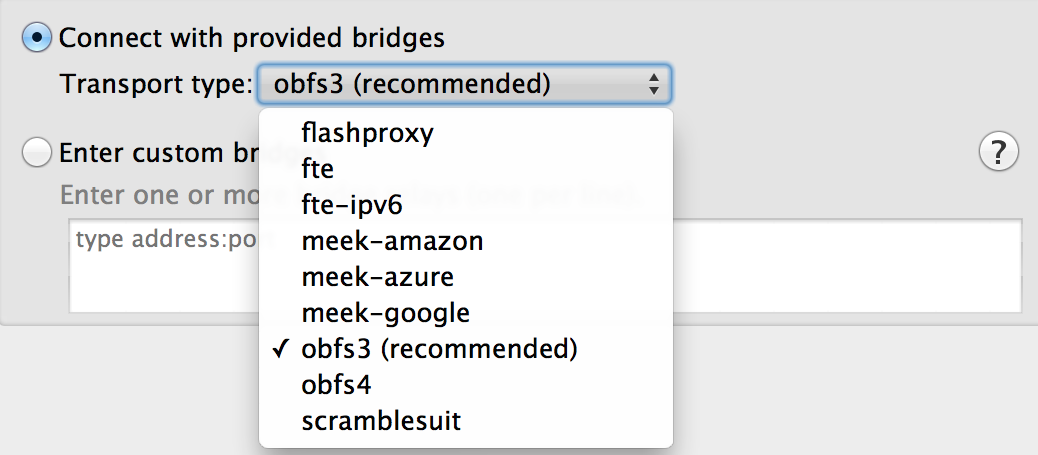
\includegraphics[width=0.5\textwidth]{bridge-options.png}
\caption{
Bridge selection options in Tor Launcher for Tor Browser~5.0.3.
Users are not familiar with the options under ``Transport type,'' which are various
built-in circumvention technologies (``pluggable transports'').
Under ``Enter custom bridges,'' there is a space to paste in
a bridge line, obtained out of band.
The ``Help'' button displays instructions on obtaining
bridge lines. 
}
\label{fig:bridge-options}
\end{figure}

In addition to Tor-specific components, a proxy may be necessary to connect 
outside the local network in certain managed environments, such as corporate or university networks.
Configuring a proxy requires providing the proxy protocol, IP address, port, and additional optional
fields. There is no assistance or automation with this process. The user must locate the 
proxy information and correctly input this information. 
  
%Technically the Tor client, pluggable transport bridge, and proxy are all
%proxies. In this paper, ``proxy'' refers to a local, ordinary unobfuscated proxy such
%as a SOCKS or HTTP proxy. An important distinction is that the local proxy lies within the 
%censor's control.

\subsection{Connecting to Tor}
There are many valid configuration settings to connect to the Tor network.
For instance, a user who does not need a bridge or proxy 
can connect to Tor with a bridge and proxy, provided that they have been configured correctly. 
The minimum amount of configuration required, therefore, the set of valid configuration settings,
vary depending on the censorship environment. In the worst case, users must know or find out:\\

\begin{itemize}
	\item{Whether their Internet connection is censored} 
	\item{Whether the Tor network is censored by their ISP}
	\item{Which hard-coded bridges work in their country} 
	\item{If no hard-coded bridges work, how to get custom bridge information and connect to it} 
	\item{Whether a proxy is required to access the Internet}
	\item{If a proxy is required, and if so, the proxy settings}
\end{itemize}

Uncensored users and users in censorship environments that do not explicitly 
block Tor do not require a bridge or a proxy and can bypass these steps in the configuration process.
Users in censorship environments that explicitly block Tor but have not blocked the 
hard-coded bridges in the Tor Launcher source code are required to use a 
hard-coded bridge or custom bridge to connect to Tor. Users in a censorship environment that has explicitly 
blocked Tor relays and hard-coded bridges are required to configure a meek bridge (which 
routes traffic through content delivery networks and therefore resists blocking through collateral damage) or 
configure a custom bridge to connect to Tor.

\subsection{Motivation} 
%Tor's anonymizing functionality also circumvents censorship. Using Tor for censorship circumvention became sufficiently common that many countries attempt to block Tor for this reason~\cite{winter2012great}. Today, Tor explicitly provides support for censorship circumvention through a network of unlisted relays as entry points into the Tor network, various methods of obfuscation to make connections to the Tor network less obvious, and advanced techniques to resist blocking.
 
%This is the first user study that investigates the usability of Tor as a censorship circumvention tool. Our experiments are both a case study observing users circumvent censorship and a step toward helping current Tor users by making censorship circumvention easier. All Tor users benefit from improving the configuration interface, and thereby increasing the adoption of Tor as a censorship circumvention tool. Users who successfully use Tor to circumvent censorship are provided with extra security features that other censorship circumvention tools do not provide, while users who use Tor as an anonymity system benefit from an increased number of overall users on the Tor network~\cite{dingledine2006anonymity}.

\section{Scope}
\label{sec:scope}
%insert explanation into why we did what we did here. 

For our experiments, we use instrumented versions of Tor Browser~5.0.3, 
the most recent stable release at the time~\cite{torbrowser-503}.
Though there were new releases during the experiments,
we used the same version across all participants to not introduce
confounding factors.

For both user studies, we simulated three censorship environments,
which we refer to as E1, E2, and E3, which are in  the order of increasing severity.
We designed the environments to be representative
of what, in our estimation, are important real-world
cases of censorship. They are not intended to imitate
any particular country's censorship environment.\\

\begin{description}
\item [E1: Mild censorship.]
(Representative of countries such as France and Australia.)
The E1 environment only blocks some websites,
as if by DNS poisoning.
We blocked subdomains of torproject.org
and wikipedia.org.
(The participants' main goal in the experiment was to read a page on en.wikipedia.org.)
To succeed in this environment,
participants only had to click ``Connect'' on the first screen;
additional configuration was optional.

\item [E2: Intermediate censorship.]
(Representative of countries such as Tunisia.)
The E2 environment blocks websites as in E1 and
additionally blocks IP addresses of public Tor relays
and directory authorities, simulating a censor who knows
about circumvention and tries to stop it.
In this environment, simply clicking ``Connect'' does not work;
participants had to select a built-in bridge
(any type other than ``flashproxy'' would work).
A custom bridge would work but was not necessary.

\item [E3: Comprehensive censorship.]
(Representative of countries such as China and Syria.)
The E3 environment blocks websites and Tor relays like E1 and E2
and additionally blocks built-in default bridge IP addresses in the Tor Browser source code.
To succeed in this environment, participants had to select
one of the ``meek'' built-in bridges (no other type of hard-coded bridges would work)
or acquire their own custom bridge and enter it manually.
\end{description}

\smallskip

Table~\ref{tab:environments} summarizes our simulated censorship
environments. We used features of the Windows operating system 
to implement the above blocking behaviors.
To simulate website blocking, we added entries to the hosts file,
mapping domain names to the address 127.0.0.1.
We used Windows Firewall rules for IP address blocking.

\begin{table}
\centering
\begin{tabular}{r c c c}
& E1 & E2 & E3 \\
% \noalign{\hrule}
websites blocked & X & X & X \\
public relays blocked & & X & X \\
default bridges blocked & & & X \\
\end{tabular}
\caption{
Summary of our simulated censorship environments.
E1 only requires participants to click ``Connect'';
E2 requires selection of a built-in bridge;
and E3 requires selection of a specific type of built-in bridge,
or manual configuration of a custom bridge.
E2's blocking is a superset of E1's;
similarly E3's is a superset of E2's.
}
\label{tab:environments}
\end{table}

\section{Qualitative Analysis of the Existing Interface (Study 1)}
\label{sec:qualitative}

We ran a qualitative, exploratory user study to gain an 
understanding of how users interact with the configuration interface and
what common problems may be. We did this by observing participants using 
the interface to circumvent censorship and interviewing them about
their experience.  Our observations during this study guided us in
redesigning the interface and provided hypotheses to test in our quantitative study.

\subsection{Inspection}
We used a combination of usability inspection methods~\cite{nielsen1994usability}
to prepare for the user study. Two researchers conducted a pluralistic 
walkthrough and stepped through various censorship
scenarios, discussing which elements would be involved for that use case, and walking 
through the configuration process. After compiling all the possible paths through the 
interface, researchers performed feature inspection, listing sequences of features used 
to accomplish typical tasks and taking note of long sequences or cumbersome
steps. In addition, we performed a heuristic evaluation to mark
likely causes of confusion for users during our study. 

\subsection{Recruitment}
Using established practices from the field of user experience research~\cite{howmanyusers},
we recruited 16 participants across the three censorship environments:
5~in E1, 5~in E2, and 6~in E3.
We pre-screened~\cite{screening} our participants for diversity of gender, age, technical expertise,
and self-reported familiarity with Tor in each simulated censorship environment for our summative
usability test~\cite{summative}. 

We recruited our users from Craigslist, vaguely asking to evaluate a piece of software. 
The recruitment text can be found in Appendix~\ref{qualitative-recruitment}. The recruitment posting contained a 
SurveyGizmo online survey that collected their demographics, technical expertise, and familiarity with Tor.
The complete prescreening survey can be found in Appendix~\ref{qualitative-prescreening}.  
We selected participants in each censorship environment to have at least one person who has never heard of Tor, 
at least one person who has only heard of Tor, and exactly one person who has previously used Tor. We tried to evenly distribute any participants who had technical
expertise or used particular security tools throughout the censorship environments. 

Of our 16 participants, 53.3\% were male. 
Ages ranged from 20 to~62 years
($\mu = 24.5$, $\sigma = 12.6$). 
93.3\% of our participants had at least
a college education.
4 had used Tor before;
5 had heard of Tor but not used it;
and the remaining 8 had never heard nor used it.


\subsection{Procedure}
The one-hour, single-participant procedure begun when a participant entered a small 
room with a single computer, which is equipped with Tor, Chrome, Firefox, Internet Explorer, and VLC.
Each participant is informed of the risks and purpose of the study.
A researcher informed the participant of the simulated censorship environment and
instruct them to visit sample blocked and unblocked websites
in a standard browser (Appendix~\ref{qualitative-script}). 
This shows participants what a blocked site looks like in a browser. 
Then, the participant was asked to complete a worksheet that gives information
on their censorship environment and instructed them
to visit one blocked website and one non-blocked website (Appendix~\ref{participant-worksheet}).
The worksheet informed the participant that the network is censored,
but did not give details of what services and websites are specifically blocked.
Participants were able to visit the unblocked website using any familiar browser,
but had to configure Tor Browser in order to visit the blocked website.
 
For the blocked website, we used the main page of Wikipedia,
and for the unblocked site we used the CNN homepage.
We chose these two sites because of their likely familiarity to web users;
our goal was to evaluate the user interface, not to test users with a browsing task.
After instructions, the researchers stepped out of the room.There was no interaction
between the participant and researcher for the rest of the session.
Researchers watched a live video of each participant's screen from another room
and saved the videos for review; the resulting videos and summaries
are available from our project page.
Participants had an average of 45 minutes to complete their worksheet. 

After participants completed the browsing tasks or ran out of time,
we interviewed them about their experience and
took notes of the questions and answers.
We asked questions asking about their general experience, 
interface features they found confusing, and feedback for improvements (Appendix~\ref{interview-questions}). 
We followed up with specific questions prompted from watching their screen. 
This was to verify any hypotheses we had (e.g. ``they did not know what an ISP was'').
We paid each participant~\$30 for their time. 

\subsection{Results} 
We discuss six common challenges our participants encountered during the configuration process.
Participant quotations come from live transcription during the post-experiment interview
and are not necessarily verbatim.\\

\begin{description}
\item {\bfseries Users did not understand what proxies, bridges, and pluggable transports were.}
Most participants, including those pre-screened for high technical ability and previous experience with Tor, were not familiar with the vocabulary.

\smallskip
\pquote{P2}{I don't know what any of those [list of bridges] means, or what that [proxy] means at all.}
\smallskip
\pquote{P3}{The vocabulary is really challenging, for someone not doing IT work.}
\smallskip

\item {\bfseries Users did not know if they should connect directly or configure a connection.}
Participants incorrectly determined that a blocked torproject.org website meant that Tor relays were censored, configuring bridges and proxies when they did not need to. Other participants tried a direct connection because they did not know what to do, but configuring their connection seemed hard. 

\item {\bfseries Users did not know how to choose which bridge and pluggable transport to use.}
On the bridge configuration screen, participants were confused by the names of the bridge transports. The most common behavior was to configure with the recommended bridge option (obfs3). If the recommended one did not work, participants did not know how to choose another. 

\smallskip
\pquote{P8}{I have no clue what's the difference between flashproxy, fte, etc. I need to know why the built-in ones aren't working. And why do I need a custom bridge if there are options built in?}
\smallskip
%\pquote{P7}{Since it (obfs3) said recommended, it helped actually, and I selected it because it was chosen. I saw the custom bridges option, but I didn't know what to enter there so I went with this (obfs3).}

\item {\bfseries Users did not know when they are wrong.}
Unfortunately, many mistakes did not result in error messages, but warnings that went unnoticed.
When participants did encounter an error message, they did not understand what errors meant (Fig.~\ref{fig:error}).

\item {\bfseries Users assumed they are wrong when they are right.}
The progress bar has a bug that causes it to update only when the level of progress increases.
If progress bar reaches a 90\% and fails, the next attempt have regressed to 0\% and remain there until the progress surpasses 90\%. Due to this, participants assumed that their subsequent attempts were wrong, even if they were right.

\smallskip
\pquote{P1}{It was hard to figure out if the progress bar wasn't moving because the connection was censored, or if it was just slow.}
\smallskip
\pquote{P16}{There doesn't seem to be a timeout on any of this stuff. Am I waiting long enough? It should work immediately.}
\smallskip

\item {\bfseries Users assume that proxy is required after a failed connection.}
All of our participants who failed to connect (5 of 16) failed for this reason. Many mistakenly assumed that they needed a proxy upon failure, because the interface redirects to the proxy screen (the last screen) after failure. 

\smallskip
\pquote{P15}{I didn't know if this computer had any proxy information. I wasn't able to find it if it did.}
\end{description}

From interviewing our participants, we found that these challenges are the result of these underlying causes: \\

\begin{description}
\item {\bfseries Users do not know how to connect to Tor.} Participants did not know the difference between a direct connection and an indirect connection to the Tor network or the difference among bridges, pluggable transports, and proxies. Participants did not know how to configure these network components without explicit additional instructions. 
\item {\bfseries Feedback is too technical, missing, or misleading.} Participants did not know when they failed, since certain mistakes do not trigger error warnings or timeouts (i.e. a syntactically correct but invalid proxy). If participants did see an error message, they did not understand it. The progress bar bug also caused users to wrongly assume they were not making progress since it did not give feedback on subsequent attempts. 
\item {\bfseries Users do not understand censorship circumvention cues.} With enough technical background, there are  signals to what components are necessary and unnecessary. A connection to the Internet indicates that no proxy is required. A failed direct connection indicates a blocked Tor relay. A failed hard-coded bridge connection indicates a blocked bridge relay. However, the average user does not understand these signals.
\end{description} 

The challenges users faced in the qualitative experiment and the respective underlying causes are used as feedback for redesigning the configuration interface. 

\begin{figure}[t]
  \centering
    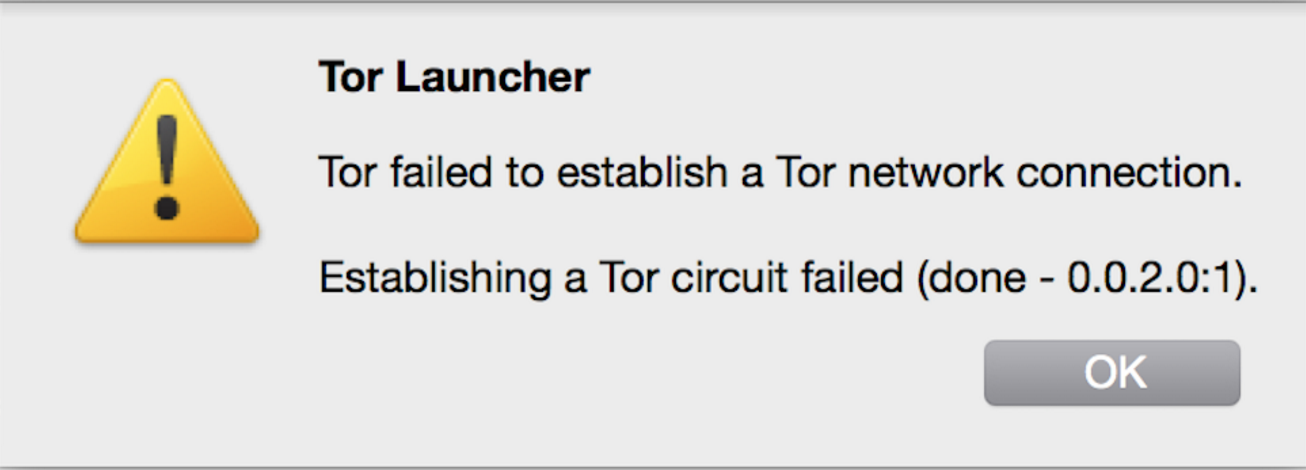
\includegraphics[width=0.5\textwidth]{error.png}
    \caption{An example of a technical error message which our participants did not understand.}
\label{fig:error}
\end{figure}

\section{Redesigning the Configuration Interface}
We make ten changes to the Tor launcher configuration interface to help users connect to Tor. Since users did not know how to connect to Tor, we added advice where our users have previously struggled. Specifically, the following three changes were made to give users more information in during configuration: \\

\label{redesign} 

 \begin{figure*}[t]
	\centering
		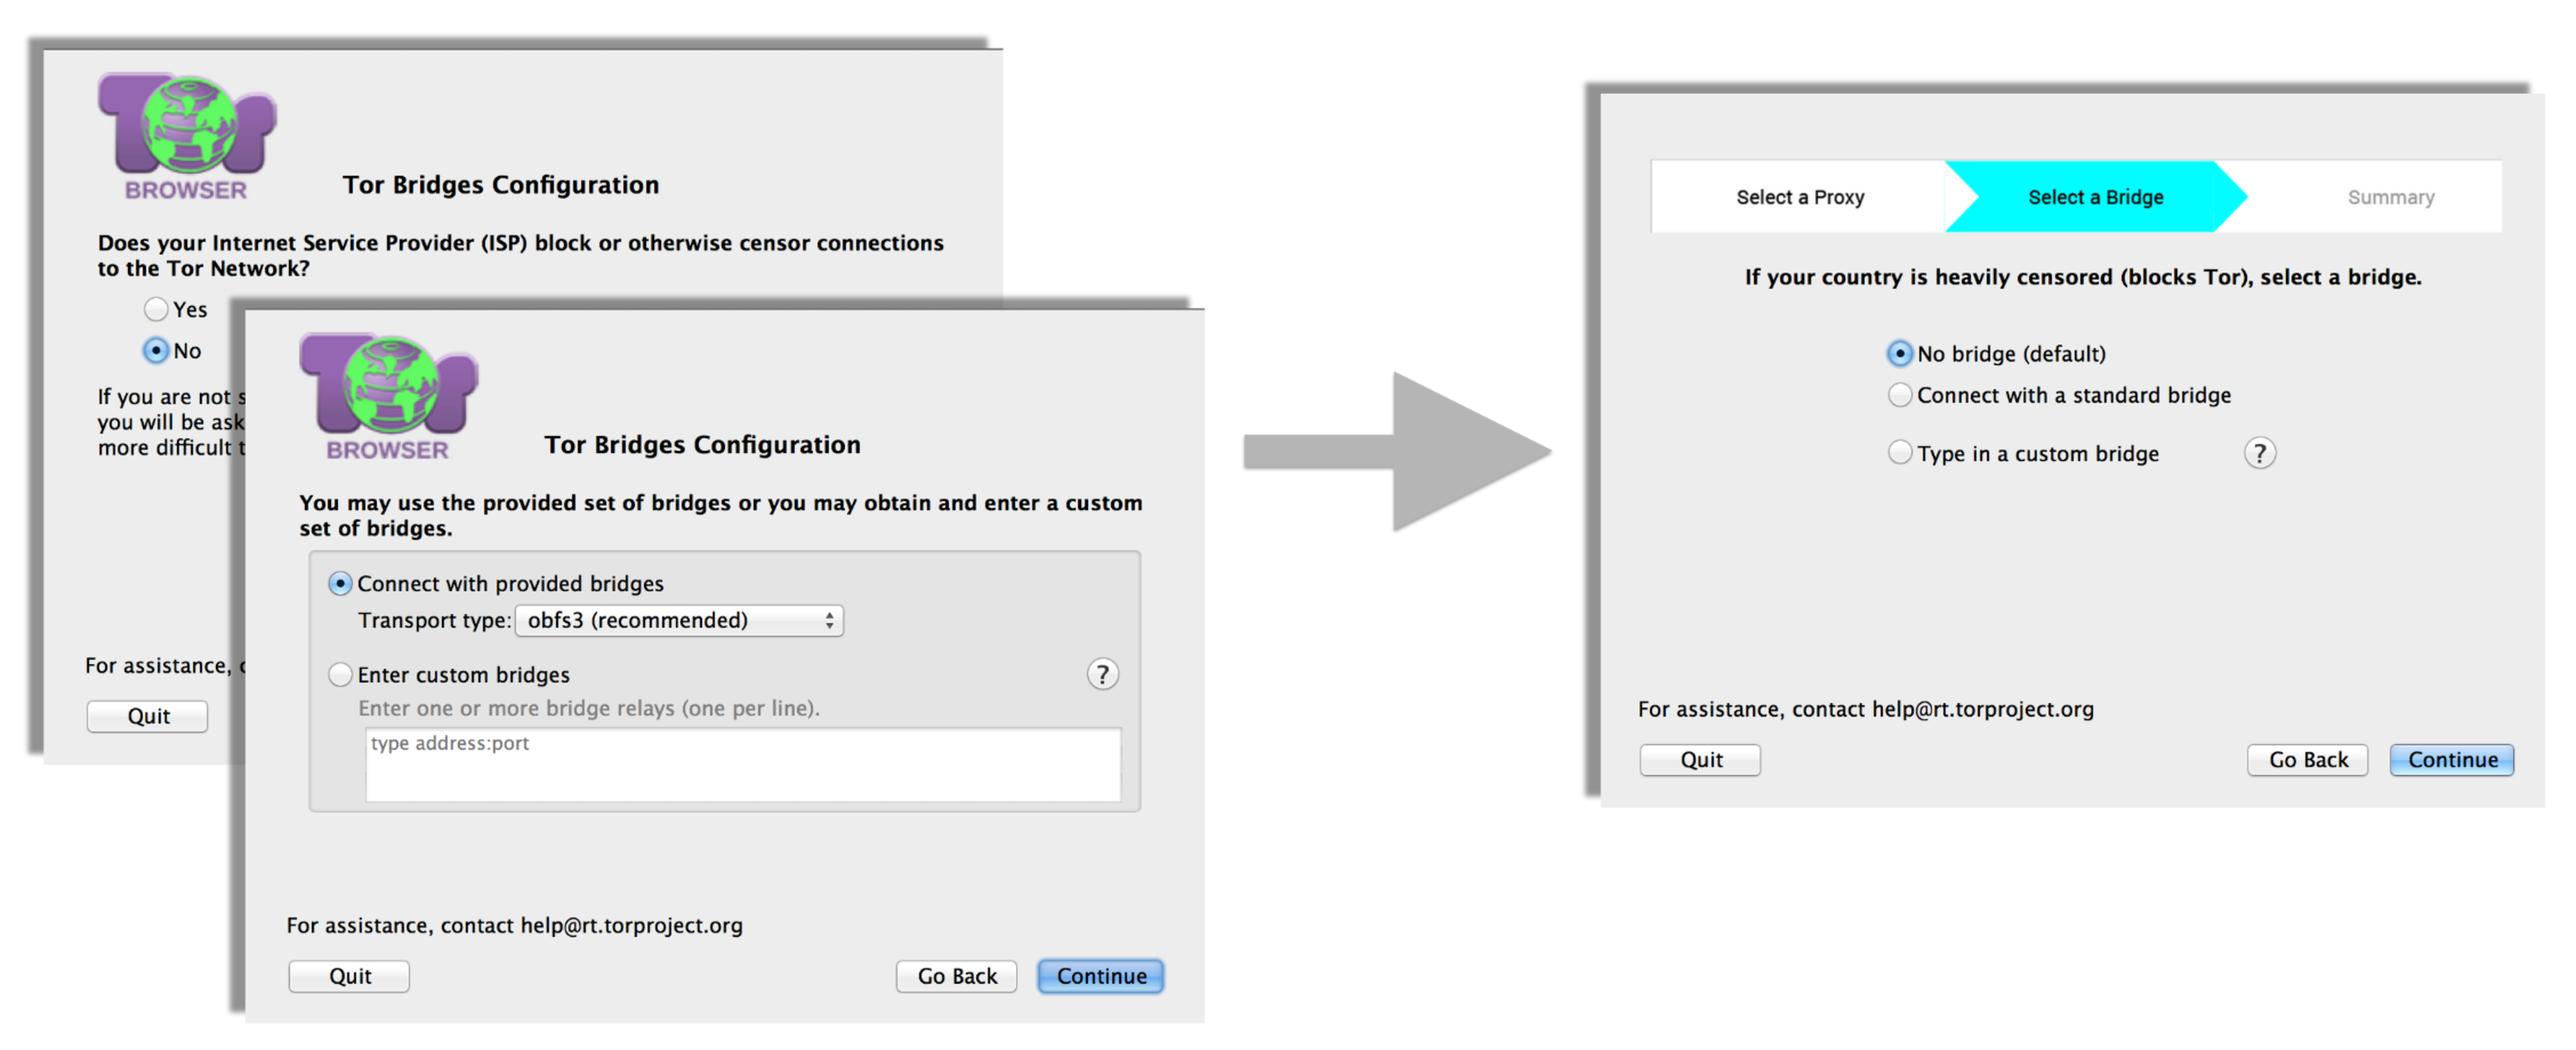
\includegraphics[width=.8\textwidth]{bridge-screens.pdf} 
		\caption{In the OLD interface, users are asked, ``Does your Internet Service Provide (ISP) block or 
		otherwise censor connections to the Tor Network?'' (B1). A ``Yes'' determines that a bridge should 
		be configured and directs to the bridge configuration screen (B2). 
		The NEW interface gives users advice on configuring bridges
		while giving the option of not configuring a bridge, on one screen (B).} 
\end{figure*} 

\begin{figure*}[t]
	\centering
		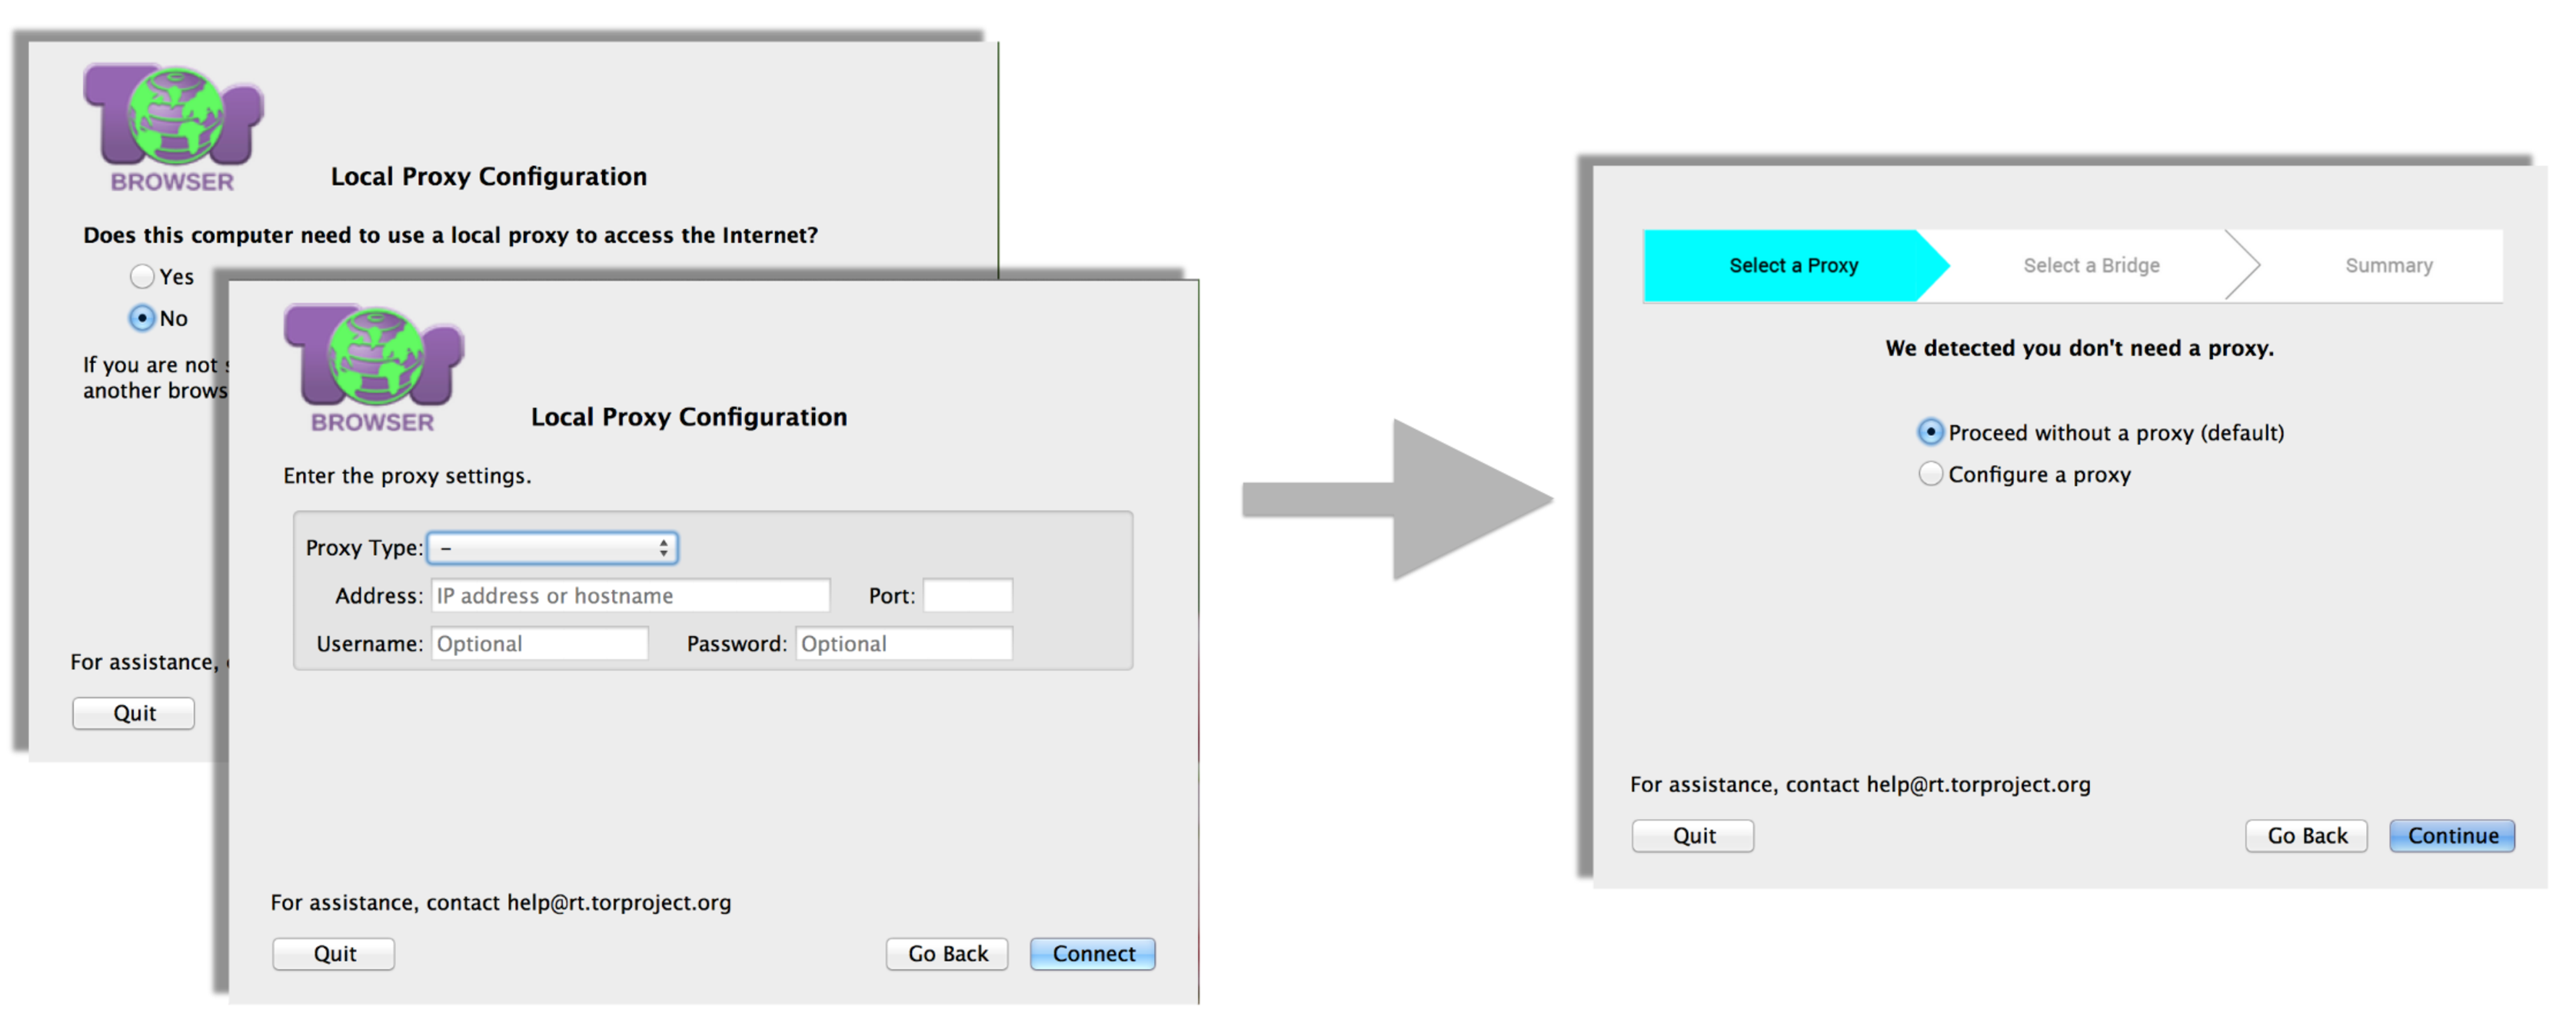
\includegraphics[width=.8\textwidth]{proxy-screens.pdf} 
		\caption{In the OLD interface, users are asked, ``Does this computer need a local proxy to connect
		to the Internet?'' (P1). A ``Yes'' determines that a proxy should be configured and directs to the 
		proxy configuration screen (P2). The NEW interface checks the local machine's proxy settings,
		and informs the user whether a proxy is required, and if so, what those settings are (P).}
\end{figure*}

\begin{figure*}[t]
\centering
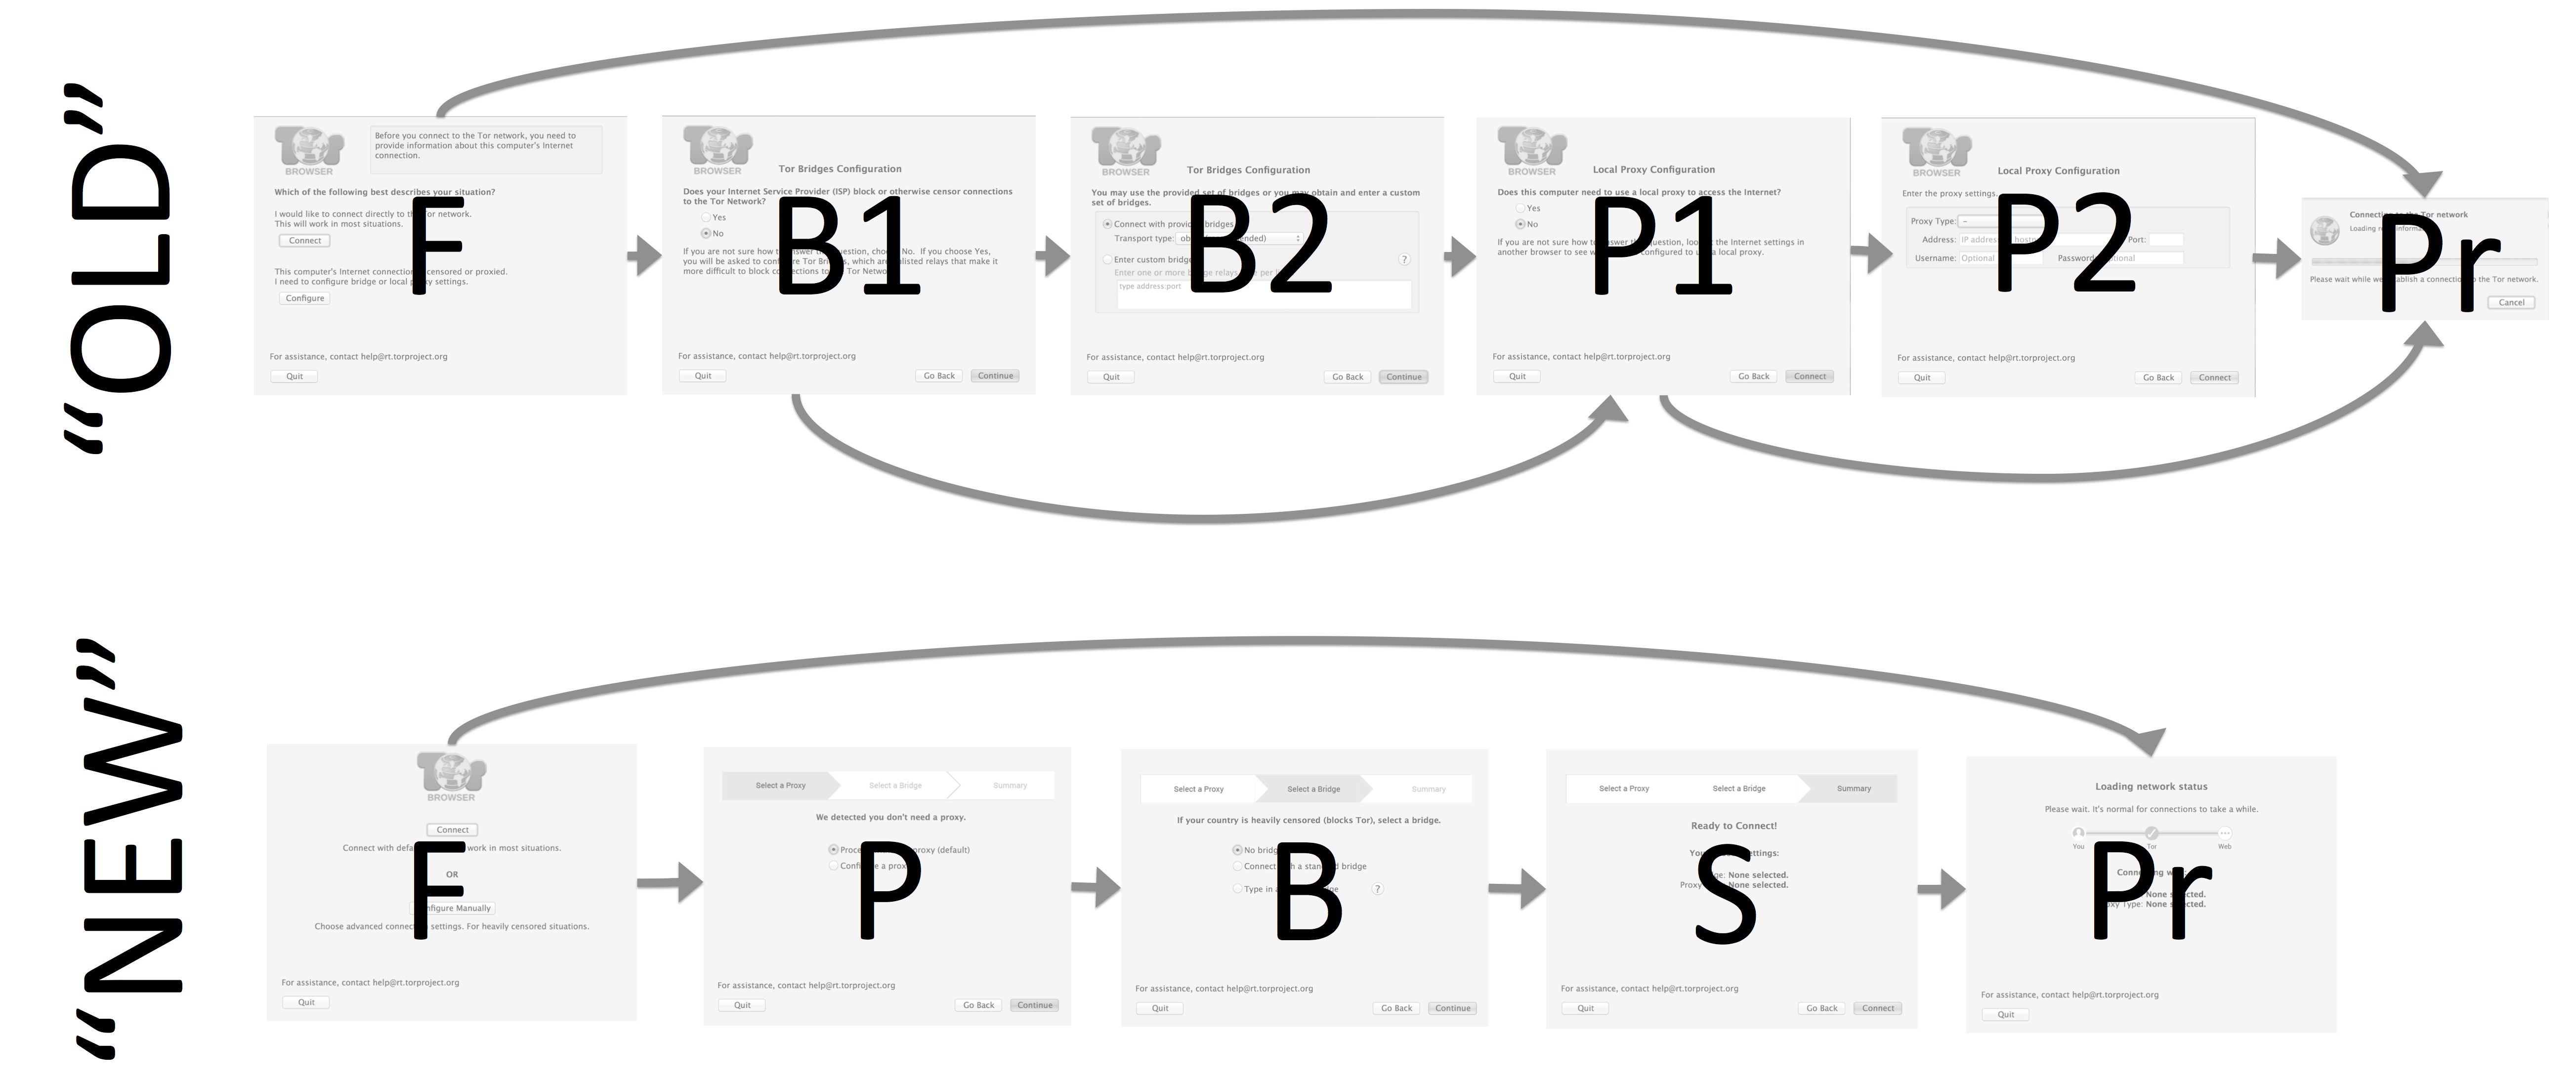
\includegraphics[width=.85\textwidth]{old-and-new-flows.png}
\caption{
Comparison of user flow in the OLD and NEW interfaces.
We collapsed the two bridge screens into one 
and also collapsed the two proxy screens into one.
We swapped the order of the bridge and proxy configuration
so it matches the order of network components (compare with Fig.~\ref{fig:topology}).
We added a summary screen as a last step before initiating a connection.\\
\textbf{F}: first screen;
\textbf{B/B1/B2}: bridge screens;
\textbf{P/P1/P2}: proxy screens;
\textbf{S}: summary screen;
\textbf{Pr}: progress bar.
}
\label{fig:flow}
\end{figure*} 

\begin{enumerate}
\item Added instructions on what to try next on errors. When an error occurs, text advice on what to try next is shown to the user to help them recover from the error. The advice may be to try the connection again, to choose a different bridge, or to try a connection without a proxy. 
\item Added guidance on choosing between connect and configure. Before, the interface only informed users that the connect option worked some of the time, but did not specify why that was so. We labeled the configure option as a manual option  specifically for users in heavily censored environments.
\item Added explicit advice on choosing bridge transports. Users did not know which bridges to choose if they were in E3, which requires users to choose a meek or custom bridge. We added text that advises users to try a meek bridge if obfs3 does not work.
\end{enumerate} 

Users found the feedback to be more confusing than helpful, since error messages were technical and progress bar was misleading. We make the following changes to make feedback insightful and reflective of system state:\\ 
\begin{enumerate}
\setcounter{enumi}{3}
\item Progress bar feedback is accurate.  We fixed the bug that caused the progress bar to not update on subsequent attempts. What users now see on the progress bar reflects the reality of the progress. 
\item Made the interface text less technical. We made the text more task-centric by focusing on instructing users through the configuration process. Since users generally did not understand the technical concepts sufficiently to influence their decisions, we think giving direct guidance is a better option. 
\item Added system status visibility. Before beginning any connection attempt, a summary screen displays the current bridge and proxy settings. The same information is shown on the progress screen while the connection is in progress. We switched the continuous progress bar to a discrete checkpoint-based progress indicator that shows the network components involved in connecting to the Tor network.
\end{enumerate}

Our users had little technical background. We made the following changes to make the interface more compatible for the average user: \\

\begin{enumerate}
\setcounter{enumi}{6}
\item Eliminated technical questions.  We removed the gating questions that determined whether a bridge and proxy should be configured, which were highly technical and challenging for users to answer. This are two fewer screens in the revised interface. 
\item Added auto-detection of proxies. In principle, the interface can guess whether a proxy is needed by scanning the operating system configuration. This purely local detection does not carry any risks nor reveal to network eavesdroppers that the user is using Tor. (We simulated the auto-detection by hard-coding the fact that a proxy was not required.)
\item Switched ordering to configure proxies first. To build users' mental models, network components are now configured in a topologically sequential order, resembling Fig.~\ref{fig:topology} and the new progress screen. Previously, proxies were put after bridge configuration because only a small fraction of users require proxies. With auto-detection, configuring a proxy before a bridge burdens users less than before.
\end{enumerate}

These changes result in a redesigned interface which we refer to as NEW. Note that the new interface preserves all the functionality of the old interface and still allows users to have control over their own network traffic. 

\section{Evaluation Criteria}
\label{sec:eval}
Our user studies evaluated two versions of the Tor Launcher interface.
The first, which we have labeled OLD in our figures and tables,
is the current version being distributed with Tor Browser.
The second, NEW, is the prototype that we designed
in order to provide better usability. Below are the empirical and 
heuristic evaluation criteria we use to assess the interfaces. 

Our empirical evaluation criteria for the Tor Browser configuration
interface are based on common metrics that measure ease of use: \\

\begin{enumerate}
    \item {\bfseries Success rate:} what percentage of users can successfully connect to Tor in a given condition. This measures how many users are able to configure their connections with the interface. 
    \item {\bfseries  Time to completion:} how long it takes between program startup and a successful Tor bootstrap, which includes time spent searching online for help and waiting for the connection to bootstrap. This measures how much time is required for a user to connect to the Tor network. 
    \item {\bfseries Active configuration time:} how much time a user spends actively configuring network components to connect to Tor, which only includes time spent interacting with the interface, excluding the time waiting for the connection to bootstrap. This measures how much of the time spent connecting to the Tor network was spent configuring versus waiting. 
\end{enumerate}

An ideal interface maximizes the amount of people that successfully connect to the Tor network, while minimizing the time it takes to connect to the Tor network. A trade-off may be required between the total amount of time it takes to connect to Tor and the amount of time users interact with the interface. For instance, a  process with a balanced amount of user input may be faster than a naive but completely automated process.

\section{Quantitative Analyses of the Interfaces (Study 2)}
\label{sec:quantitative}
Having identified problems with the existing interface
and made changes to ameliorate them,
we quantify the existing problems
and the impact of our changes with a study involving a larger number of users.
We split participants by simulated censorship environments,
and between old and new interfaces.

\subsection{Setup}
We ran our experiment at <redacted>.
%Xlab~\cite{xlab}, the Experimental Social Science Laboratory at the University of California, Berkeley. 
<redacted> %Xlab 
has 36 Windows~7 laptops, separated by cubicle walls. 
Though Tor Browser runs on other operating systems,
testing was only done on Windows, as a byproduct of using <redacted>. %Xlab. 

We augmented the interfaces with instrumentation 
to log every meaningful interaction
(button presses, menu selections, screen changes).
We wrote scripts to automatically set up the simulated censorship environment, install necessary software, 
start the video recording, and save the logs and videos.
We recorded the participants' computer screens
throughout the experiment to capture non-interface activity such as 
web searching and inspection of system networking settings.

\subsection{Recruitment}
We recruited 124 participants, about 20 for each
condition. We recruited half of our users from Craigslist, and half of our participants from 
the <redacted> %Xlab 
participant pool. Although <redacted> %Xlab 
participants are not limited to <redacted> %UC Berkeley 
students and staff,
a majority of the participants are from campus. For this reason, we chose to recruit 
half of our participants from Craigslist to ensure a diverse set of participants. 
The recruitment text vaguely suggests testing a piece of software, and does not require
that users provide information in advance (Appendix~\ref{quantitative-recruitment}). 
Out of our 124 participants, 59 were recruited from the <redacted> %Xlab 
pool and the other 65 were
recruited from Craigslist. Ages ranged from 18 to~68 years
($\mu = 28.9$, $\sigma = 12$). 56.8\% were male and 
84.8\% of our participants had at least a college education.

\subsection{Procedure}
The one-hour, multi-participant procedure began when all participants sat at their
respective computers in <redacted>. %Xlab. 
Each computer was equipped with an instrumented old or new version
of Tor Browser, Chrome, Firefox, Internet Explorer,  Chrome, and VLC (for screen recording).
Each computer was assigned one of the six conditions in the beginning of the study. Participants
were assigned to a simulated censorship environment combination at random. 

A researcher informed the participants that they are in a
simulated censorship environment, instructed them to visit a sample blocked website on a 
non-Tor browser of their choice to illustrate the situation, and asked them to 
complete a worksheet that asks to visit one blocked website (Appendix~\ref{quantitative-script}). 
To mirror the qualitative study, we chose Wikipedia's featured article of the day 
as the blocked website to visit on their worksheet. 

After instructions, researchers maintained minimal interactions with the participants, 
only answering logistical questions.
The participants did not know the details of their censorship environment,
only that they are being censored. Participants had 40 minutes to configure Tor Browser to 
circumvent the simulated censorship and visit the blocked website. 

After users completed the browsing tasks, they took a short exit survey (Appendix~\ref{quantitative-exit-survey})
that collected their demographics. All users were instructed to sit until the end of the experiment,
regardless of when they had completed their task. After the 40 minutes, 
participants were officially informed that their time was up, and were given their payment of 
\$30 for their time. 

\subsection{Results} 
The possible interface version and environment combinations resulted in 6 experimental conditions. We recruited 124 participants to aim for about 20 participants per condition. We filtered participants who downloaded their own version of Tor Browser or did not sign the consent form, resulting in 114 participants. Table~\ref{table:participant-summary} summarizes the rate of success, time to success, and active time for our participants' by condition. 

\begin{table}
\centering
% Do not edit this file. Edit info.R instead.
\begin{tabular}{l r r r r r}
& \multicolumn{2}{r}{success rate} & \multicolumn{1}{r}{median time} & \multicolumn{1}{r}{median} \\
& \multicolumn{2}{r}{after 40 minutes} & \multicolumn{1}{r}{to success} & \multicolumn{1}{r}{active time} \\
\noalign{\hrule}
E1-NEW & 19/19 & 100\% & 0:20 & 0:06 \\
E1-OLD & 19/19 & 100\% & 1:01 & 0:24 \\
E2-NEW & 18/18 & 100\% & 3:22 & 0:40 \\
E2-OLD & 16/19 & 84\% & 5:00 & 2:04 \\
E3-NEW & 13/19 & 68\% & 20:25 & 1:56 \\
E3-OLD & 10/20 & 50\% & 40:08 & 9:06 \\
\end{tabular}

\caption{
A summary of participants' success in circumventing censorship
given their simulated censorship environment and version of Tor. Those who
failed to connect successfully were assigned the maximum time of 40:08.
}
\label{table:participant-summary}
\end{table}

\subsubsection{Rate of Success} 
49 of 56 (88\%) participants with the new interface successfully connected to Tor, while 45 of 58 (78\%) participants with the old interface did. Due to the limited number of participants, this difference is not large enough to rule out the possibility of random chance being the cause for the difference. Appendix~\ref{stat-tests} details the methodology for the statistical tests used in this paper. 

%\begin{figure}[t]
%\centering
%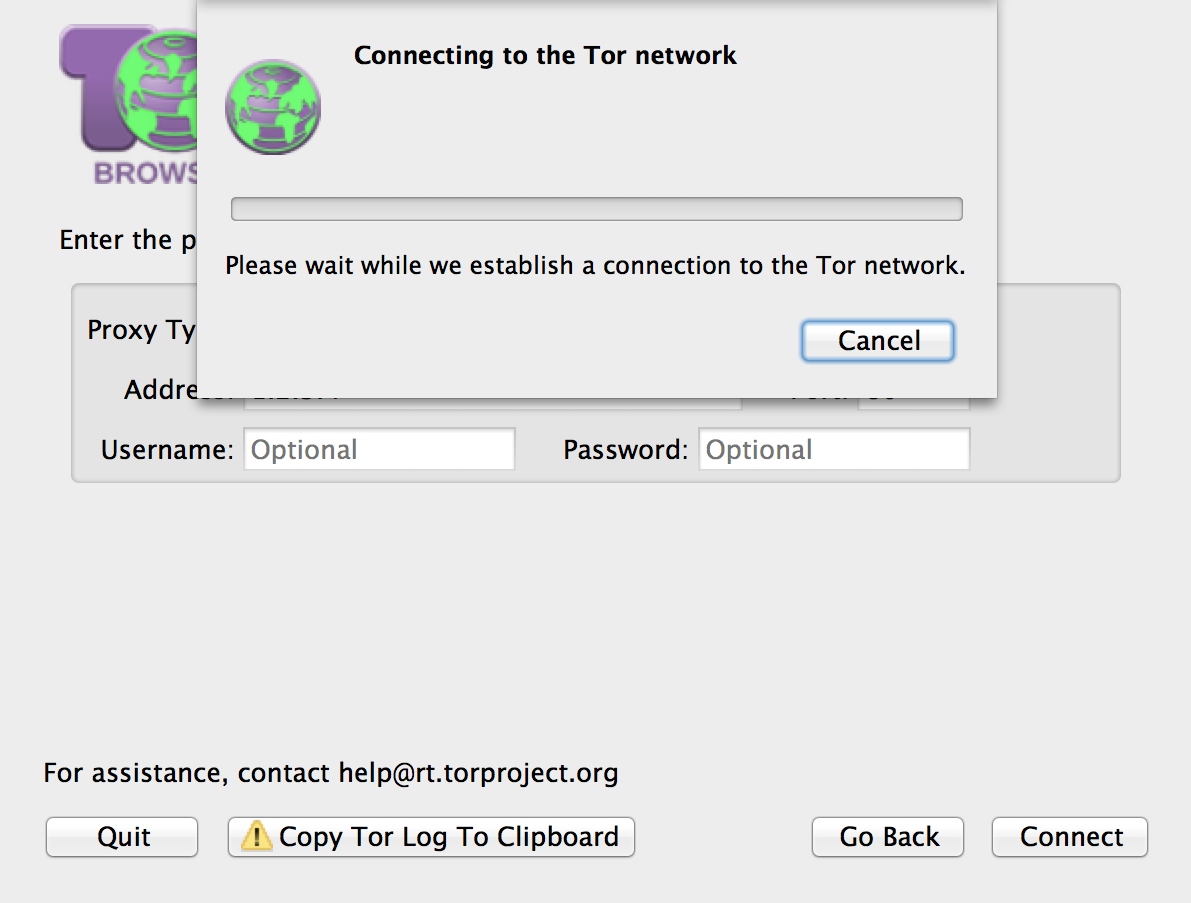
\includegraphics[width=.5\textwidth]{warning.png}
%\caption{
%A screenshot of the interface with the ``Copy Tor Log to Clipboard'' button, 
%which appears silently and does not interrupt the progress bar. 
%This warning was generated by entering in syntactically correct but invalid proxy settings,
%a mistake that prevents users from ever connecting to the Tor network. 
%Users are never directly notified of this error through an error message or a timeout message.
%Our participants made this error during our experiments, along with others that they were not notified about. 
%}
%\label{fig:warning}
%\end{figure}

%\begin{figure}[t]
%\centering
%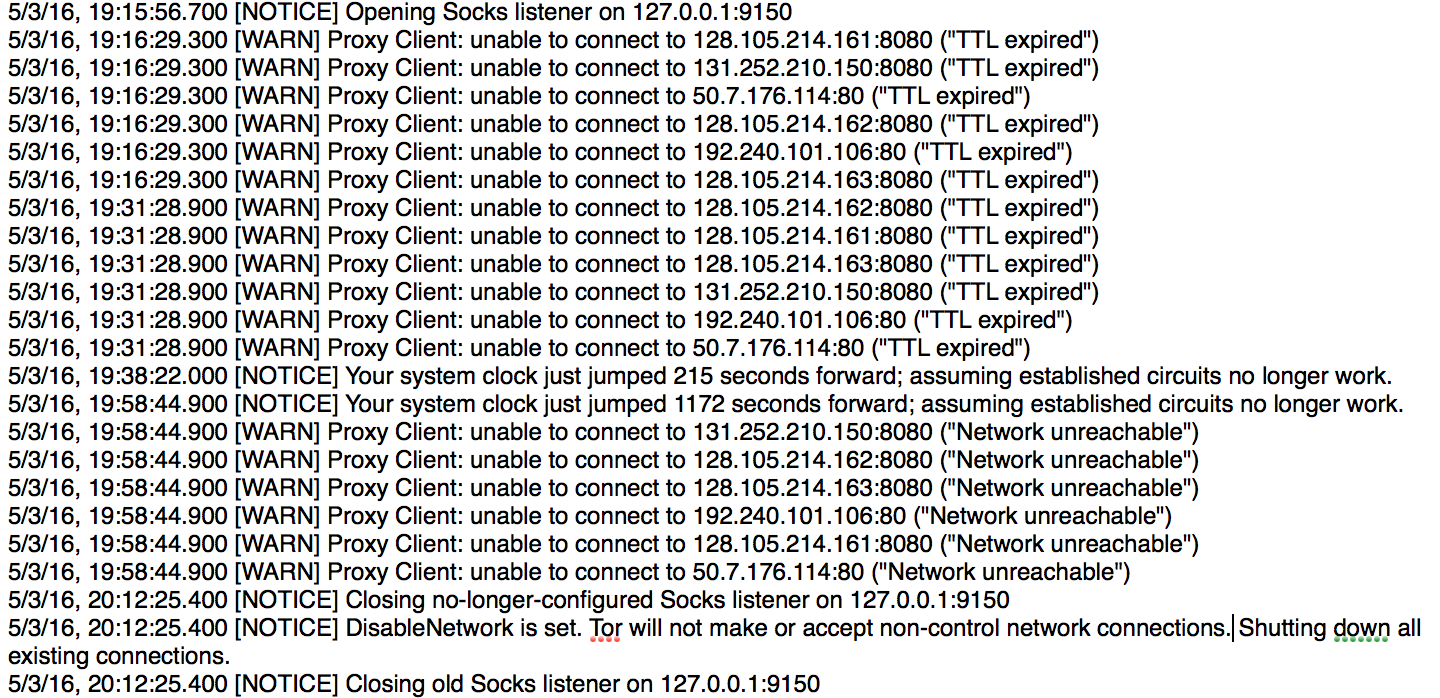
\includegraphics[width=.5\textwidth]{log-messages.png}
%\caption{
%The last 24 of 45 log lines that users receive after clicking clicking the ``Copy Tor Log to Clipboard'' button. 
%These log lines were the result of entering in syntactically correct but invalid proxy settings,
%a mistake that prevents users from ever connecting to the Tor network. Understanding the Tor logs require
%technical expertise from the user to understand the logs, diagnose the problem, and formulate next steps.
%}
%\label{fig:warning_log}
%\end{figure}
%
%We believe that the added advice on what to try next on error messages would have improved the rate of success. However, only 1 of 116 participants saw an error during the experiment. The old interface warned users on some mistakes (i.e. entering in a syntactically correct but invalid proxy settings) rather than displaying an error message. When a user receives a warning, a button that says ``Copy Tor Log to Clipboard'' silently appears at the bottom of the interface (Figure~\ref{fig:warning}). To see the log messages, users must click on the button, open up a text editor, and paste the log messages. The log messages require the user to understand the log, diagnose the problem, and formulate next steps (Figure~\ref{fig:warning_log}).
%
%That participant was using the new interface and was told that the bridge configuration was the source of the error. The participant heeded the interface's advice to reconfigure the bridge options. But since most participants did not see any error messages, any effects they may have had on success rates are not reflected in our results. The addition of a summary screen did cause behavioral changes (13\% of participants saw their current settings, then went back and adjusted them), but this behavioral change did not have a statistically significant impact on success rates. 

We added preemptive advice to the bridge configuration screen to first try an obfs3 bridge and then a meek bridge, but we suspect that most participants did not benefit from this advice since participants did not think to adjust their bridge settings upon failure. Of the 75 participants that failed to connect on the first attempt, 15 participants with the new interface and 13 participants with the old interface went back to the bridge screen and chose another hard-coded bridge. 10 of 15 in the new interface chose a meek bridge as their next bridge whereas 5 of 13 in the old interface chose meek as their next bridge, but we cannot claim choosing meek bridges is a direct result of our advice.

Table~\ref{tab:attempts-bridge-proxy} shows the configuration settings of the first successful connection in each environment and interface combination.We only consider the first successful connection since many of our curious participants tried many different settings to investigate if they will work, even after they had completed the task. Recall E1 does not require users to configure a bridge, E2 requires users to configure any bridge, and E3 requires users to configure a meek or custom bridge. Note that only four of the hard-coded bridges were used to connect successfully for the first attempt were the recommended bridge and the required bridges to succeed in E3.

Our participants did not optionally configure a bridge in E1 or configure a non-recommended bridge in E2. This suggests that users will not configure optional components or deviate from the recommended settings unless necessary. If the intent of the recommendation is to get as many users as possible to use the recommended bridge, this is a positive result. If the intent of the recommendation is to give pointers when users are stuck but allow the users to make their own bridge choices to diversify active transports, this is a negative result. 

Only two participants chose to configure a custom bridge. Both of these participants sent an incorrectly formatted request to the automatic bridge responder, which did not reply with custom bridges as a result. Appendix~\ref{custom} shows the malformed requests. These two participants failed to connect to the Tor network. 

\begin{table}
\centering
% Do not edit this file. Edit attempts.R instead.
\begin{tabular}{r c c c c c c}
& \rotatebox{90}{E1-NEW} & \rotatebox{90}{E1-OLD} & \rotatebox{90}{E2-NEW} & \rotatebox{90}{E2-OLD} & \rotatebox{90}{E3-NEW} & \rotatebox{90}{E3-OLD} \\
no bridge, no proxy & 17 & 13 &  &  &  &  \\
obfs3, no proxy & 2 & 6 & 18 & 16 &  &  \\
meek-amazon, no proxy &  &  &  &  & 7 & 4 \\
meek-google, no proxy &  &  &  &  & 5 & 4 \\
meek-azure, no proxy &  &  &  &  & 1 & 1 \\
no bridge, 3rd-party proxy &  &  &  &  &  & 1 \\
DNF (did not finish) &  &  &  & 3 & 6 & 10 \\
\end{tabular}

\caption{
Bridge--proxy combinations that led to the first successful bootstrap
in each environment and interface.
Most E1 participants used a direct connection,
but a few tried a built-in obfs3 bridge.
All the E2 participants who succeeded,
did so with obfs3 (the recommended bridge type)---none tried
a different bridge before obfs3.
All of the successful E3 participants but one
used one of the meek bridges.
The remaining E3 participant succeeded in an unexpected way:
by searching the web for an open proxy and configuring it
as the proxy setting.
}
\label{tab:attempts-bridge-proxy}
\end{table}

\subsubsection{Time to Success} 
Time to success is defined as the time until the first successful connection to Tor. Non-finishing participants are assigned the maximum experiment time of 40:08.  Our changes to the interface had a significant impact in reducing the time participants took to successfully connect to Tor (Mann--Whitney $Z = -1.84$, $p = 0.0328$, $r= 0.172$; see Appendix~\ref{stat-tests}). The simulated censorship environment also had an impact; the more difficult the censorship environment, the longer participants took to configure their connection (Kruskal--Wallis $\chi^2 = 80.5$, $\mbox{df} = 2$, $p < 10^{-15}$). 
Table~\ref{table:participant-summary} shows the median active times and Figure~\ref{fig:time_to_success_clamped} shows their distribution.

\begin{figure}[t]
\centering
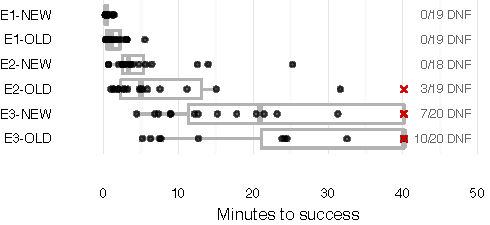
\includegraphics{time_to_success_clamped}
\caption{
Time to first success, by censorship environment and interface.
The dots show the raw completion times,
while the boxplots show the medians and interquartile ranges.
The ``DNF'' figures at the right show the number of participants 
who did not finish in the time allotted.
Here, non-finishing participants are assigned the maximum time of 40:08.
}
\label{fig:time_to_success_clamped}
\end{figure}

In our experiment, participants had 40 minutes to circumvent censorship. Fig.~\ref{fig:time_to_success_ecdf} shows the cumulative success rates over time. In practice, faster time to completion would mean more users will succeed, since users will give up after a while. Users in the wild will likely not be motivated to spend 40 minutes trying to configure Tor. If users were only willing to put in a minute or so of their time, users in intermediate and heavily censored environments would be unable to connect. Even if users were willing to dedicate 10 minutes to configuring their connection, most users in heavily censored environments would be unable to connect. Ideally, users should be able to connect to Tor within a few minutes, regardless of their censorship environment. We propose ideas on how to achieve this in section~\ref{recommendations}. 

\begin{figure}[t]
\centering
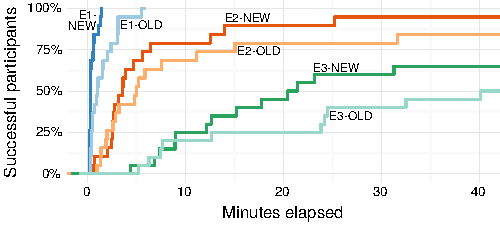
\includegraphics{time_to_success_ecdf}
../experiment/processing/time_to_success_ecdf.tex
\caption{
Cumulative success rates over time, by censorship environment and interface.
We stopped participants after 40 minutes. Here, those who did not finish were assigned
an arbitrarily high number greater than 40 minutes for the purposes of plotting. 
For example, every E1-NEW participant finished within 90 seconds,
but only 58\% of E1-OLD had finished by that time. Within 10 minutes, most
participants in E2 had finished, along with a minority of E3 participants. 
}
\label{fig:time_to_success_ecdf}
\end{figure}

\subsubsection{Active Time} 
We summarize each participant's actions throughout the experiment in Fig.~\ref{fig:all-participant-edges}.
%and summarize where they spent their time in Appendix~\ref{all-participant-times}. 
Each row in Fig.~\ref{fig:all-participant-edges} corresponds to a participant. The bar represents a path through the interface, illustrating time spent on each screen, transitions between screens, how many attempts were made, and if they were eventually successful. 

\begin{figure*}
\centering
% This is a manually edited version of the automatically generated
% all-participant-edges graphic. It is edited to have better scale labels for
% the treatments.
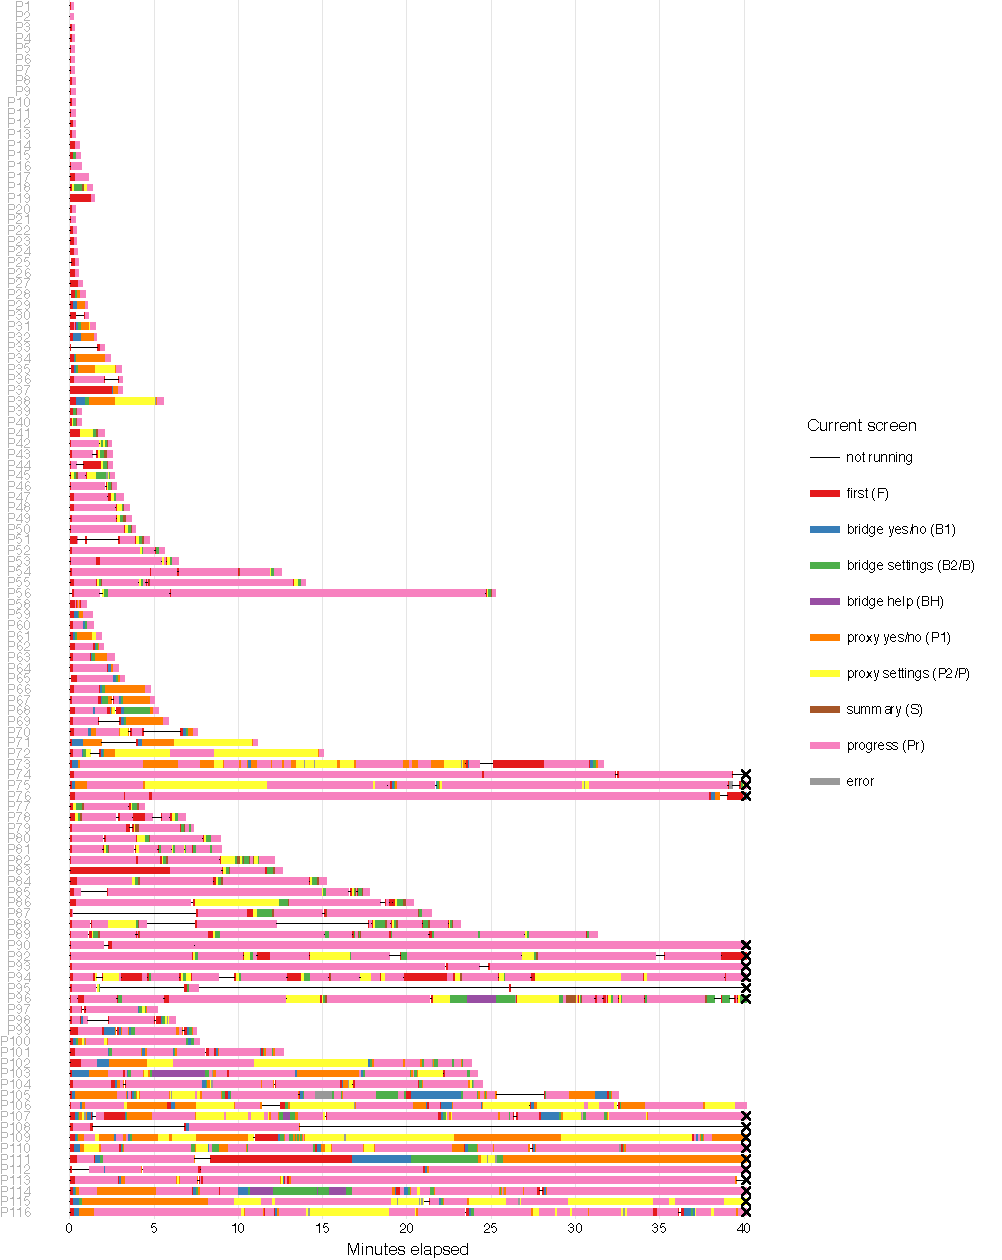
\includegraphics{all-participant-edges}
\caption{
Summary of participants' actions throughout the entire experiment.
Different colors indicate which screen was shown at each moment.
The ``not running'' times are those when Tor Launcher was closed;
i.e., a participant was doing something else
such as searching the web in another browser.
The overall length of the lines show the total time to completion,
except for those we cut off after approximately 40 minutes.
}
\label{fig:all-participant-edges}
\end{figure*}

The overall time was largely dominated by the time spent waiting to connect to Tor, rather than actively configuring the interface. With correct configurations, the bootstrap process can take up to two minutes.  With incorrect configurations, a lack of error messages on the progress screen caused some users to wait indefinitely.  Logs show that participants spent 58\% of their overall time at the progress screen. Table ~\ref{table:median_time} shows the median percentage of time spent on each screen. 

\begin{table}[t]
\centering
\begin{tabular}{l r r r r}
& First & Proxy & Bridge & Progress \\
\noalign{\hrule}
E1-NEW & 28\% & 0\% & 0\% & 60\% \\
E1-OLD & 30\% & 0\% & 0\% & 29\% \\
E2-NEW & 6\% & 5\% & 6\% & 78\% \\
E2-OLD & 7\% & 18\% & 8\% & 45\% \\
E3-NEW & 3\% & 5\% & 5\% & 77\% \\
E3-OLD & 2\% & 12\% & 6\% & 64\% \\
\end{tabular}

\caption{The median percent of time spent on each screen, which is not
necessarily the median absolute time spent on that screen. 
This percentage is computed independently for each screen; that is, a participant who spent the median percent 
of time on one screen may not be the same participant who spent the median percent
of time on other screens. Note that the time spent on the progress bar dominates the 
time spent in the interface.} 
\label{table:median_time}
\end{table}

\begin{figure}[t]
\centering
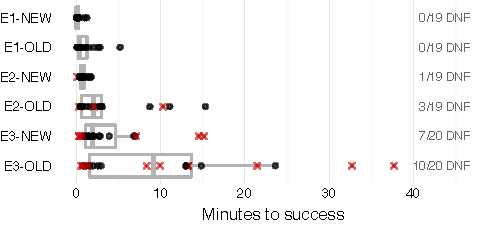
\includegraphics{time_to_success_active_clamped}
\caption{
Active time, by censorship environment and interface.
The dots show the raw active configuration times,
while the boxplots show the medians and interquartile ranges.
Here, non-finishing participants' active time was computed by
subtracting the amount of time spent on the progress screen from the 
the maximum time of 40:08.
}
\label{fig:time_to_success_active_clamped}
\end{figure}

Perhaps a more meaningful measurement is the amount of time participants actively configured their connection (Figure~\ref{fig:time_to_success_active_clamped}). We define active time as the time that participants spent interacting with the interface, excluding the time waiting for the connection to bootstrap. Active time for unsuccessful participants were calculated by subtracting the amount of time spent on the progress screen from the maximum experiment time, 40 minutes. This is an approximation, since some participants searched for help on the web after exiting the interface or on the progress screen. 

We performed a one-tailed Mann--Whitney test to compare the amount of active configuration time between participants who used the new interface and the participants who used the old interface. Our changes to the interface reduced the time participants spent configuring the interface (Mann--Whitney $Z = -3.28$, $p = 0.000516$, $r = 0.307$).  Table~\ref{table:participant-summary} shows the median active times and Figure~\ref{fig:time_to_success_active_clamped} shows their distribution.


\subsection{Discussion} 
We talk about the failure cases and behavioral trends observed in our quantitative user study and recommend some changes to the Tor configuration interface based on those observations. 

\subsubsection{Failures}
Failure is common. 17\% (19 of 114) of participants were not able to successfully connect to Tor. 63\% (72 of 114) of first attempts to connect failed and (363 of 458) of total attempts to connect failed. Reasons for failure were determined by a combination of log processing (i.e. configuration settings on attempts) and video observation (i.e. observing what they searched for online). \\ 

\begin{description}
\item {\bfseries Only connected directly (6/19).} P73, P75, P89, P91, P106, P110 tried a direct connection. When that failed, they tried the same option, over and over, no matter how many times they failed. It was common to restart the interface, check Internet settings, and wait between subsequent attempts.

\item {\bfseries Only tried recommendations (5/19).} P90, P93, P108, P111, P114, who were in E3, did not know what to do next after a direct connection and a default obfs3 bridge connection. They often tried those configurations again or gave up. 

\item {\bfseries Thought that they needed a proxy (5/19).} P74, P92, P105, P107, P113 assumed that they needed a proxy. They spent their time trying to configure a proxy, usually without trying other bridges. 

\item {\bfseries Used the bridges auto-responder incorrectly (2/19).} P94, P109, who were in E3, emailed the bridges auto-responder to get custom bridges. However, they formatted the message incorrectly and thus failed to get a response (Appendix~\ref{custom}).
\end{description}

We discarded data on participants who chose to download their own version of Tor Browser online. 5 participants downloaded their own version without trying the provided one on their desktop, while others did so after feeling frustrated with the provided version. Appendix~\ref{tor-downloads} gives the unfortunate details of where Tor was downloaded when torproject.org was blocked.


\subsubsection{Observations}
We noticed several behavioral patterns in our participants. These may or may not apply to the Tor user base.\\

\begin{description}
%connect vs configure
\item {\bfseries Users try the easy path first.} Users generally try connecting directly to the Tor network first. 81\% (92 of 114) of first attempts were to connect directly, with 52\% (48 of 92) direct first attempts from the new interface and 47\% (44 of 93) direct first attempts from the old interface. This leaks to network eavesdroppers that they are connecting to Tor.

% impacts of making the proxy page ``automated'' 
\item {\bfseries Users wasted time configuring proxies.} This confusion prevented users from configuring their bridges correctly. Participants with the new interface (which explicitly states that they did not need a proxy) spent about the same time configuring proxies as bridges, whereas users with the old interface spent about twice as much time configuring proxies than bridges. We do not understand why users with the new interface spent time configuring proxies after explicitly being told that they do not need one.

% impacts of giving people advice on which transport to choose.
\item {\bfseries The interface has a large influence on the bridges chosen.}
Participants in E3 were required to choose a particular subset of hard-coded bridges, none of which was the default bridge. After the default bridge, the most chosen bridge was the one listed first in the drop-down menu. Many bridges listed at the end of the drop-down menu were not chosen. We tried to help users by providing instructions on which bridges to choose if the default fails, but it is unclear if this advice helped. 66\% (10 of 15) participants with the new interface and 38\% (5 of 13) participants with the old interface chose meek as their second bridge.

%error messages
\item {\bfseries People saw (almost) no error messages.} Many waited for minutes at the progress screen, but never saw an error message. Error messages are intended to appear after a timeout. There were warnings, but those warnings went largely unnoticed by our participants. Across both versions of the interface, only one participant ever saw an error message. We tried to make error messages more instructive and understandable, since participants in our experiment did not encounter error messages, we cannot evaluate them. 

% progress bar
\item {\bfseries People waited a long, long time at the progress bar.}
From watching the screen capture videos, we see that some participants dutifully followed the directions to wait, while others are who are uncertain wait without taking additional actions.
\end{description}

\subsubsection{Recommendations}
\label{recommendations}
Based on our observations of general behavioral trends and common failure cases, we make the following recommendations to increase success rate and decrease overall time spent in the interface: \\

\begin{description}
\item {\bfseries Automate configuration after failure.} After one unsuccessful attempt, a user has already leaked to network eavesdroppers leaking that they are connecting to Tor. Automating the configuration process thereafter will have no increase in risk. This will specifically help users that will never try to configure their connection (the most common failure case) to succeed and drastically reduce the time spent for the 63\% of participants who failed their first attempt. Users in more comprehensive censorship environments are more likely to benefit from this, as 5\% of participants in the mild censorship environment, 84\% participants in intermediate censorship environment, and 100\% of participants in the heavy censorship environment failed the first time.
\item{\bfseries Hide infrequently used options.} Telling users they did not need a proxy was not enough to deter users from configuring a proxy. Only a small fraction of the Internet population requires a proxy to connect to the Internet. Hiding the proxy screen by default and only showing it after it has been detected as necessary might improve the user experience focusing user effort on configuring bridges.
\item {\bfseries Be explicit about recommendations.} Many do not know what to do after the recommended bridge failed. The interface should mark which bridges have been tired before and recommend the user to try another bridge. (i.e. After a user tried an obfs3 bridge, the interface updates its recommendation to a meek bridge and mark the obfs3 bridge with an ``X''.)
\item{\bfseries Set a timeout on the progress bar.} Informing users that they have failed earlier will decrease the overall time to success, create an opportunity to give suggestions, and reduce user frustration. 
\item{\bfseries Have a user-tolerant bridge auto-responder.} The bridge auto-responder responds to user requests for custom bridges. Users can make this request by emailing bridges@torproject.org with a non-empty title and ``get bridges'' in the body. Both of our users who tried to get custom bridges this way failed to format their request correctly. Having the auto-responder respond with bridges as a default or recovering from common errors (such as typing ``get bridges'' in the subject line) may help users succeed. 
\end{description} 

Although we cannot isolate their effects on users, we also recommend notifying a users with the configured settings before connecting and having a progress bar that illustrates when network component have successfully been configured or failed.

\section{Limitations} 
The configuration interface uses the native operating system's elements and their respective styling, so an interface looks slightly different across different operating systems. We only tested interface on Windows machines, which were the machines available at <redacted>. %Xlab. 
Participants who are not accustomed to Windows machines may have been slower to complete the given task, but this affected all conditions equally. 

We refreshed a list of Tor relay IP addresses and added them
to a firewall blacklist before each session.
In the first study, we neglected to block the IP addresses
of the Tor directory authorities, which are the first hosts
a client contacts when initiating a non-bridge connection.
New relays also appeared in the network on an hourly basis,
which enabled a small number of participants to succeed with
a direct connection when that configuration should have failed.
We believe this is acceptable because 
the qualitative user study was not used to quantify failures or successes, 
but to explore possible problems.
We fixed this problem in our quantitative user study by blocking the directory authorities.

%We blocked en.wikipedia.org, the target of the experiment,
%as well as other language-specific subdomains such as
%de.wikipedia.org and fr.wikipedia.org.
%We neglected, however, to block the Simple English Wikipedia
%at simple.wikipedia.org, which one participant found,
%thinking they had completed the task.
%% E2-OLD-X04-20160330-181928

Our study was conducted in a laboratory setting, which can cause our participants to be under or over-motivated. Our participants had a monetary incentive to connect to Tor, whereas a real user in a censored environment would want to reach a particular website. 

We chose to focus on more common cases, and did not simulate environments that requires users to configure a custom bridge or proxy. Although users in the wild can download interfaces that are not in their native language, we do not know how often this happens. We tested the English version of the Tor interface on English speaking participants. 

\section{Related Work}
\label{sec:related} 
There have been three published user studies on Tor. Clark et~al.~\cite{clark2007usability} examined various deployment
options for Tor Browser, such as Vidalia, Privoxy, Torbutton, and FoxyProxy, and found that none had satisfactory from a usability. Fabian et~al.~\cite{fabian2010privately} show that Tor's added
latency~\cite{dingledine2009performance} causes users
to be frustrated, cancel requests, and prevents user adoption. 
Norcie et~al.~\cite{norcie2012eliminating} found found that 
64\% of users are unable to continue with installation or browsing at least once due to difficulties.

We do not know of any published usability evaluations of
Tor Browser since the release of the 3.5 series in 2013, which introduced radical UI changes~\cite{torbrowser-35}.
The most recent effort is an unpublished pilot study by Lee and Fifield~\cite{uxsprint} 
that tested the downloading, installation, and browsing tasks in Tor Browser.  This study uncovered a number of issues~\cite{uxsprint2015-tickets},
some of which influenced changes in Tor Browser version~4.5 and later.

Previous user studies have considered the whole browsing experience,
without focusing on specific features in isolation.
Our study focuses on 
the browser's configuration interface, which guides users through setting up components required to circumvent censorship. 

\section{Conclusion} 
We conducted a series of experiments to improve the Tor Browser 5.0.3 configuration interface, focusing on users who use Tor to circumvent censorship. Since connecting to the Tor network unsuccessfully indicates to network eavesdroppers that users are connecting to Tor, the configuration process is manual to allow users to have control over the network activity. Through interviews and lab studies, we find that users have difficulty configuring network components to circumvent censorship, because they do not know how censorship or Tor works. We detail the common challenges, our changes to the configuration interface address those challenges, and the recommendations we have for Tor in this paper. 

%general advice to other censorship circumvention and call for more research 
Interacting with a censorship circumvention tool users can be a complex balance of leveraging user input for local information while accounting for user trust of the software and minimizing potential risks.
When designing censorship circumvention tools, we caution against requiring first-time users to make decisions on software-specific notions (e.g. pluggable transports for Tor), answering questions that assume technical knowledge, or manually configuring components. We encourage the use of simulated censorship environments as a tool for user testing censorship circumvention software. Not only do simulated environments avoid rerouting traffic through a censoring country's networks, their reproducibility and stability are ideal for experiments. 


%\section {Resources} 
%For additional details, such as the censorship simulation code, interview transcriptions, and logs of participant interactions, we refer you to the project repository: \\
%
%\noindent \url{https://github.com/lindanlee/circumvention-ux-tor}
%
%\section {Acknowledgments}
% Rowilma del Castillo of Xlab supported out experiment by assisting with testing, offering recruitment services, and allowing experiments after-hours. Nima Fatemi, Isabela Bagueros, Georg Koppen, and the Tor UX team have provided me with valuable feedback along the way. 

\bibliographystyle{abbrv}
\bibliography{pets2017-paper}

\appendix
\section{Alternative Approaches} 
%In principle, the process of configuring a proxy and bridge can be automated, but
%the interface eschews automatic configuration through network probing
%in favor of guided manual configuration to give users agency in configuring their connection. 
%Automatic configuration through network probing may put some users in certain regimes at risk. 
%A knowledgeable user can minimize their network trace and hide that they are connecting to Tor.
%However, this requires that the user grapple with technical concepts such as 
%bridges, pluggable transports, and proxies. Some of these concepts are specific to 
%Tor and not general concepts.

Our goal was to deploy impactful, tested changes the Tor configuration interface. In fact, Tor version~4.5 incorporated textual and navigational changes based on our redesigned interface. Throughout our experiments, we collaborated with Tor developers and focused on discovering changes that could be deployed right away. For this reason, we assumed that the configuration process will remain a manual process that requires user inputs, as it is currently deployed. However, we list some alternative approaches that seem worth exploring. \\

\begin{description}
\item{\bfseries Automate the configuration.} The most efficient way to connect as many users to the Tor network is to automatically configure their connection on start. A naive automation is to try configurations that would most likely work, in order (i.e. a direct connection, then an obfs3 connection without a proxy, then an meek bridge connection with out a proxy). This leaks to network eavesdroppers that the user is connecting to the Tor network. We do not know how much risk is associated with this approach. 
\item{\bfseries Ask about the risk.} An alternative to naive automation is to offer manual configuration to those that want to be more cautious and automatically configuring a connection for who are not at risk. The complication with this approach is that users may not be qualified to answer if they are at risk or may not trust Tor with this information. 
\item{\bfseries Ask if users know what to do.} Another alternative to naive automation is to offer manual configuration to those that know how to configure their connection and to automate the process for users who do not know how to configure their connection. This may prevent the most mistakes, but does not account for the users' risk associated with using Tor. 
\item{\bfseries Suggest configurations.} A way to help users without any automation or questions is to give users information about what would work in their country. The first page of the configuration interface can show a list of countries with a corresponding recommended configuration. This approach does not require users to answer about their risk, technical ability, or location. However, it does require that the user trust the given advice and to correctly configure their settings based on this advice. 
\item{\bfseries Assign configurations.} This is a smart way to automate connections to the Tor network. Upon start, the interface detects proxy settings and uses them, if any. Then, all users connect to bridges that will always work (such as meek bridges), which assign them a guard relay based on their location, effectively assigning bridges for the user. 
\end{description}

We believe that automation, asking about risk, and identifying struggling users could enable significant improvements to the configuration process. 

\section{Qualitative User Study Recruitment Posting} 
\label{qualitative-recruitment}
We are recruiting participants for an in-person research study at <redacted>. %the University of California, Berkeley. 
You will need to come in to our lab and perform tasks on a computer for an hour or less. You will be compensated \$30 for participating. 
No special knowledge and no technical experience is required. If you are interested, fill out the survey at \textit{<survey link>}. 

\section{Qualitative User Study Prescreening Survey} 
\label{qualitative-prescreening}
We are recruiting participants for an in-person research study at the <redacted>. %University of California, Berkeley. 
You will need to come in to our lab and perform tasks on a computer for an hour or less. You will be compensated \$30 for participating. No special knowledge and no technical experience is required.\\

\begin{enumerate}
\item{Please select when you are available. We will assign you an hour experiment time slot during one of those times.}
\item{I am able to provide my own transportation to the <redacted> %University of California, Berkeley 
campus.}
\item{Thank you for your interest! Please provide an email address where we can contact you to share more logistical details.}
\item{we are looking for a very small number of participants, so unfortunately, we may not be able to accommodate everyone who applies. Would you like us to let you know about future opportunities?}
\item{What is your gender?}
\item{What is your age?}
\item{Please select your highest completed (or current) level of education.}
\item{What is your occupation?} 
\item{Do you speak any languages other than English fluently?}
\item{If you have a personal computer, what kind do you use?}
\item{Which of the following terms have you heard of? \textit{<answer choices: a checkboxlist of the the following terms: malware, proxy services, phishing, SSL, X.511 certificates, Tor>}}
\item{How often do you use the following software or features? \textit{<answer choices: a grid of radio buttons. Software/features (rows): HTTPS on web pages, proxies or other censorship circumvention tools, virtual private networks (VPN), file or whole-disk encryption, anonymity systems (e.g., Tor), email encryption (e.g., PGP), chat or instant messaging encryption, voice communication encryption. Frequency (columns): never, less than once a month, a few times a month, several times a week, daily.>}}
\end{enumerate}
Thank you for filling out this form. You are now done!

\section{Qualitative User Study Introduction Script} 
\label{qualitative-script} 
Imagine you live in an oppressive country that censors part of the Internet. We have simulated this in the laboratory by blocking certain websites and services.  The purpose of this experiment is to evaluate the use of Tor browser, which is a browser that can circumvent censorship and let you visit blocked websites. Currently, torproject is blocked (you can check this by going to torproject.org on a standard browser, like Firefox, Chrome, or Internet Explorer). 

To circumvent censorship successfully, you will need to set up Tor browser correctly and use it to get to Wikipedia. If you are able to reach the website, then you know that you have successfully circumvented censorship. Fill out the question on the worksheet. This isn't intended to be hard, just write what you see. We want to just check you saw the website. 

Before you start, do you have any questions about what you are asked to do? 

\section{Participant Worksheet Text} 
\label{participant-worksheet}
Imagine you live in an oppressive country that censors part of the Internet. We have simulated this in the laboratory by blocking certain websites and services. The purpose of this experiment is to evaluate the use of Tor browser, which is a browser that can circumvent censorship and let you visit blocked websites. For instance, www.torproject.org is blocked. Check this by going to the site on a standard browser, like Firefox, Chrome, or Internet Explorer. It will fail to load, when you can visit other sites.

To complete this worksheet, you will need to set up Tor browser (on your desktop) correctly and use it to get to blocked site. If you can visit wikipedia, then you know that you have successfully circumvented censorship.

\section{Post-Experiment Standard Interview Questions}
\label{interview-questions}
We asked our participants these questions after they were given time to configure Tor Browser. \\

\begin{enumerate}
\item{Can you talk us through what you did along with what you were thinking at the time?}
\item{What was most challenging part of connecting?}
\item{Were there any unfamiliar terms?}
\item{How did you decide which options to choose?}
\item{What did you think about using Tor?}
\item{What is one change you would recommend?} 
\item{Did you need any additional information?} 
\end{enumerate}  

In addition to these questions, we asked our participants about specific questions based on their observation, usually regarding a specific choice in action, a particular screen they seemed stuck on, and any errors they encountered during the configuration process. 

\section{Quantitative User Recruitment Posting}
\label{quantitative-recruitment}
We are recruiting up to 40 participants for a user study at <redacted>. %UC Berkeley. 
The experiment will involve basic Internet browsing tasks. You are not eligible if you have participated in our previous sessions.\\

\indent Payment: \$30 Amazon gift card\\
\indent Duration: 1 hour \\
\indent Where: <redacted> \\ %Xlab at Hearst Memorial Gymnasium\\

\textit{<list of sessions>}\\

To be eligible, you must be an adult (18 or older). This is to comply with university policies on research. 

If you are interested: 1. Email <redacted> %lnl@berkeley.edu 
with the sessions you are able to attend. We will confirm your participation and assign you a session. 
2. Come to <redacted> %Xlab 
at the appointed time for the experiment.

\section{Quantitative User Study Introduction Script} 
\label{quantitative-script} 
Imagine you live in an oppressive country that censors part of the Internet. We have simulated this in the laboratory by blocking certain websites and services.  The purpose of this experiment is to evaluate the use of Tor browser, which is a browser that can circumvent censorship and let you visit blocked websites. Currently, torproject is blocked (you can check this by going to torproject.org on a standard browser, like Firefox, Chrome, or Internet Explorer). 

To circumvent censorship successfully, you will need to set up Tor browser correctly and use it to get to Wikipedia. Tor is already installed for you. On the desktop, you should see a globe icon that says ``Start Tor Browser.'' If you are able to reach the website, then you know that you have successfully circumvented censorship. Fill out the question on the worksheet. This isn't intended to be hard, just write what you see. We want to just check you saw the website. 

Afterward, we ask you to take a short survey to collect some information about you. The link is also on your worksheet.
We will give you time to complete this task. If you finish early, we ask that you sit at your desk until the remainder of the hour. Since we are recording your screen, we ask that you don't do anything personal afterward, like checking your email.

Before you start, do you have any questions about what you are asked to do? 

\section{Quantitative User Study Exit Survey} 
\label{quantitative-exit-survey}
We'd like to know more about you.  All of your answers will be stored separately from any identifying information in order to protect your confidentiality.

This survey is part of a research project being conducted by the <redacted>. %University of California, Berkeley. 
If you have any questions about your rights or treatment as a research participant in this study, please contact the <redacted>'s %University of California at Berkeley's 
Committee for Protection of Human Subjects at 510-642-7461, or email 
<redacted>. %subjects@berkeley.edu. 
If you agree to participate, please click Next below.\\

\begin{enumerate}
\item{What is your participant ID? (This can be found on the sticker on the left hand corner of the desk you are currently sitting at.)}
\item{What is your gender?}
\item{What is your age?}
\item{Please select your highest completed (or current) level of education}.
\item{What is your current occupation?}  
\end{enumerate}

Thank you for participating in our experiment. You are now done! Please sit at your desk for the remainder of the experiment. Our researchers will formally announce the end of the experiment. 

\section{Statistical Tests} 
\label{stat-tests}
From our measurements, we observe that participants with the new interface 
have a higher rate of success, succeed in less time, and configure their interface in less time. 
We do not find that the increased rate of success with the new interface or the decreased time to success with the new interface significant. That is, random chance can account for the difference. 
We do find the the decreased active configuration time to be significant. 
We describe the methodology for the statistical tests used in this paper to determine the impact of the interface on success rate, time to success, and active time. 

%success rate and version
Each participant had a boolean variable indicating a successful connection to Tor. Rates of success were calculated by dividing the number of participants who succeeded the condition over the total number of participants in the condition. This gave us six rates of success. E1-NEW, E2-NEW, and E3-NEW rates of success were compared against E1-OLD, E2-OLD, and E3-OLD.  We used a Pearson's Chi-squared test to test the significance of success rates. The difference between success rates of participants with the new interface and participants with the old interface was not significant ($X^2 = 0.0126$, $df = 2$, $p = 0.994$).

%time to success and version
Time to success was measured as the time from the participants started the Tor launcher interface to the first successful bootstrap to the Tor network. This measurement was 1) non-normal and heavily right-tailed since participants were less and less likely to succeed as time went on and 2) right-censored at 40 minutes, the maximum time of the experiment. Because of the right-tailed nature of the data, we used a one-tailed Mann--Whitney test. Because the Mann--Whitney test does not account for right-censored data, we assigned the participants who did not succeed the maximum time of 40 minutes for the purpose of this test. We find the difference of times to success between participants with the new interface and participants with the old interface to be significant ($ Z = -1.84$, $p = 0.0328$, $r= 0.172$). 

%active time and version
Active configuration time was measured as the time the participants spent in the Tor launcher interface, except for the time spent the progress screen. For our participants who did not succeed to connect to Tor, subtracted the time spent on the progress screen from the maximum experiment time of 40 minutes. This measurement was also 1) non-normal and heavily right tailed and 2) impacted by right-censored measurement of time to success. Because of the right-tailed nature of the data, we used a one-tailed Mann--Whitney test. We find the difference of active configuration times between participants with the new interface and participants with the old interface to be significant ($Z = -3.28$, $p = 0.000516$, $r = 0.307$).


\end{document}
